\documentclass[11pt,a4paper]{article}
\usepackage[margin=2.4cm]{geometry}
\usepackage[T1]{fontenc}
\usepackage{lmodern}
\usepackage{amsmath,amssymb}
\usepackage[numbers,sort&compress]{natbib}
\usepackage{xcolor}
\usepackage{graphicx,booktabs}
\usepackage{amsthm}
\usepackage{tikz}
\usetikzlibrary{arrows.meta,fit,backgrounds,shapes.geometric}
\newtheorem{proposition}{Proposition}
\usepackage[colorlinks=true,linkcolor=blue!50!black,citecolor=blue!50!black,urlcolor=blue!50!black]{hyperref}

\title{Reading Folded Hands:\\Opponent Modelling in Heads-Up Limit Hold'em}
\author{Catalin-George Tisca}
\date{}

\newcommand{\hy}[1]{-}
\begin{document}
\maketitle

\begin{abstract}
To beat a poker opponent you need to know how they play, but you only see
their cards when a hand is played to the end. We model the opponent with a
\emph{Bayesian network}: their hidden cards and the public cards decide how
strong their hand is, and strength, the situation at the table and their
current playing style decide what they do. After every action the network
gives a probability for each pair of cards they might hold. The network also
shows that hands where the cards stay hidden can still be used for learning,
while learning only from shown hands is biased. On $120{,}000$ logged hands
between poker programs, where every card is known, this makes the learned
behaviour about 80 times more accurate and improves decisions. On $87{,}428$
hands between humans, it finds that people change style about every 50 to 65
hands, while programs almost never do.
\end{abstract}

\section{Introduction}

In heads-up limit Texas Hold'em, two players each get two private cards and
share five public cards, dealt over three rounds (flop, turn, river) with
betting before and after each. A hand ends when someone \emph{folds}, and no
cards are shown, or at the \emph{showdown}, where both hands are shown. The best
programs already play close to an unbeatable equilibrium~\cite{bowling2015}. To
win more, a player has to exploit how one particular opponent deviates from it,
and learn this mostly from hands where the opponent's cards are never seen.

Bayesian networks have been used for this since the Bayesian Poker
Player~\cite{korb1999,nicholson2006}. Most such models learn only from
showdowns~\cite{korb1999,nicholson2006,terry2005}; models that also use folded
hands~\cite{southey2005,ponsen2008} assume an opponent who never changes; and
changing opponents have been tracked only in tiny games~\cite{bard2007}. Our
network combines both: it reads the cards through all rounds of a hand, and lets
the opponent's style change between hands. Because competition logs record
every card~\cite{phhdata}, we can check it against the truth. We show that
\begin{itemize}
  \item learning only from showdowns is badly biased, and using folded hands
        fixes it (Sections~\ref{sec:learning} and~\ref{sec:results});
  \item one model per opponent reads cards better and makes better river
        decisions, but does not yet win more over whole hands;
  \item the network detects a change of opponent within about ten hands, and
        humans change style far more often than programs.
\end{itemize}

\section{The model}\label{sec:model}

We describe one opponent from the seat of the other player, the
\emph{observer}, using the probability vocabulary of~\cite{bertsekas2000}. A
\emph{session} is the sequence of hands against the same opponent.
Figure~\ref{fig:net} shows the network.

\begin{figure}[t]
\centering
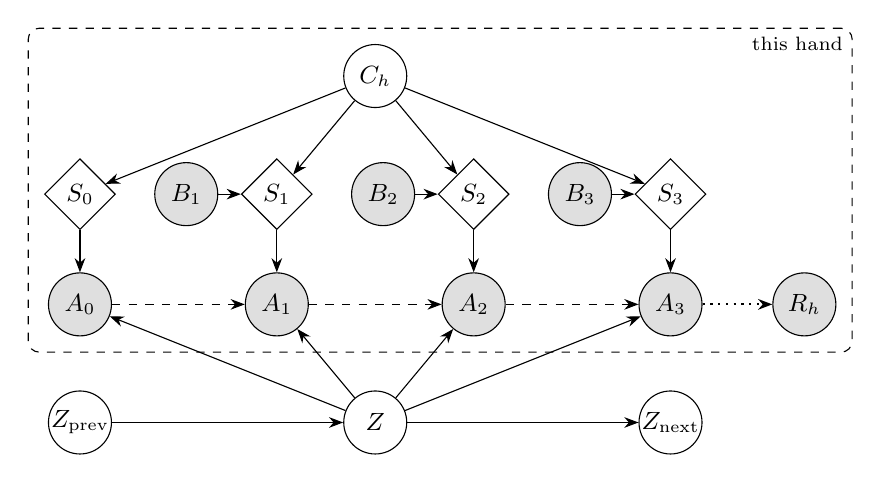
\begin{tikzpicture}[>={Stealth[length=1.8mm]},
  hid/.style={circle,draw,minimum size=8mm,inner sep=0pt,font=\small},
  obs/.style={circle,draw,fill=gray!25,minimum size=8mm,inner sep=0pt,font=\small},
  det/.style={diamond,draw,minimum size=9mm,inner sep=0pt,font=\small}]
  \node[hid] (C) at (3.75,0) {$C_h$};
  \foreach \t in {0,1,2,3} {
    \node[det] (S\t) at (2.5*\t,-1.5) {$S_{\t}$};
    \node[obs] (A\t) at (2.5*\t,-2.9) {$A_{\t}$};
    \draw[->] (C) -- (S\t);
    \draw[->] (S\t) -- (A\t);
  }
  \foreach \t in {1,2,3} {
    \node[obs] (B\t) at (2.5*\t-1.15,-1.5) {$B_{\t}$};
    \draw[->] (B\t) -- (S\t);
  }
  \foreach \t/\u in {0/1,1/2,2/3} { \draw[->,dashed] (A\t) -- (A\u); }
  \node[obs] (R) at (9.2,-2.9) {$R_h$};
  \draw[->,dotted,thick] (A3) -- (R);
  \node[hid] (Z) at (3.75,-4.4) {$Z$};
  \node[hid] (Zp) at (0,-4.4) {$Z_{\text{prev}}$};
  \node[hid] (Zn) at (7.5,-4.4) {$Z_{\text{next}}$};
  \draw[->] (Zp) -- (Z);
  \draw[->] (Z) -- (Zn);
  \foreach \t in {0,1,2,3} { \draw[->] (Z) -- (A\t); }
  \begin{scope}[on background layer]
    \node[draw,rounded corners,dashed,fit=(C)(S0)(A0)(A3)(B1)(R),inner sep=2mm,
          label={[font=\scriptsize,anchor=north east]north east:this hand}] {};
  \end{scope}
\end{tikzpicture}
\caption{The network. Inside a hand (dashed box), the opponent's cards $C$ and
the board $B$ give a strength $S$ for each round, and the strength drives the
actions $A$. The style $Z$ also drives the actions and can change from hand to
hand. Grey: what the observer sees. Diamonds: computed, not random. Whether
the cards are shown ($R$) is decided by the actions alone.}
\label{fig:net}
\end{figure}

\paragraph{What is in a hand.} The opponent holds a pair of cards $C$, one of
1326 possible pairs. Before any betting, every pair that does not clash with a
card we can see is equally likely. On each round the pair has a
\emph{strength} $S$ from 1 (weakest) to 8 (strongest): we rank all pairs by
how likely they are to win on the current board~\cite{johanson2013} and cut the
ranking into eight equal groups. Strength is recomputed every round, so a pair
can be weak on the flop and strong on the river; this is what ties the rounds
together. The opponent's action $A$ is fold, check/call or bet/raise, taken in
a \emph{situation} $X$: the round, whether they face a bet, how many bets have
been made, and their position (80 situations in all).

\paragraph{How the opponent acts.} The opponent's behaviour is a table
\[
  \theta_{z,x,s}(a)=P(\text{action }a\mid\text{style }z,\ \text{situation }x,\
  \text{strength }s),
\]
for example ``in this situation, with a strength-2 hand, this opponent bets
10\% of the time''. The \emph{style} $Z$ is hidden; it stands for how the
opponent is playing right now, say cautiously or aggressively. From one hand to
the next the style switches with a small probability $\varepsilon$ and
otherwise stays the same, so the styles form a Markov chain.

\paragraph{Reading the cards.} Bayes' rule gives the probability of each pair
$c$ after the actions seen so far:
\[
  P(c\mid\text{actions})\ \propto\
  \prod_{\text{actions}}\theta_{z,x,\,\text{strength of }c}(a).
\]
In words: a pair becomes more likely if it would have made the observed
actions likely. If the opponent raised on the river, strong pairs gain and weak
pairs lose. We do this exactly for all 1326 pairs after every action. The style
is tracked in the same spirit, hand by hand: each style gains weight when it
explains the hand well.

\paragraph{Decisions.} From the card probabilities we get $q$, our chance of
holding the better hand. If the opponent bets $b$ into a pot of $P$, calling
risks $b$ to win $P$, so calling pays off on average exactly when
$q>b/(P+b)$.

\paragraph{Explaining a decision.} Since everything is a probability, the
network can say why it recommends an action, in three ways.
\begin{itemize}
  \item \emph{How sure?} The table $\theta$ is learned from a limited number of
        hands, so it is uncertain. We redraw plausible tables many times and
        recompute the decision; the \emph{certificate} is the share of draws
        that agree. Near 100\% the advice is safe; near 50\% it is a coin flip.
  \item \emph{Which action mattered?} Each opponent action gets a score: the
        log of how much more likely it is if the opponent is strong than if
        they are weak. The scores add up exactly to the total change in belief,
        so they show which action moved it most.
  \item \emph{What would change my mind?} We swap one opponent action at a
        time and report the smallest change that flips the advice, e.g.\ ``had
        they raised before the flop instead of calling, call''.
\end{itemize}

\section{Learning and data}\label{sec:learning}

\paragraph{Folded hands can be used.} When a hand ends in a fold we do not see
the opponent's cards, so we do not guess them: we add up the probability of the
observed actions over every pair they could have held. This is safe for a
simple reason. The cards stay hidden \emph{because} of a fold, and the fold
itself is seen. So the fact that the cards are hidden tells us nothing beyond
the actions we already have, and averaging over the possible pairs loses no
correctness.
\begin{proposition}\label{prop:ignore}
If whether the cards are shown depends only on the observed actions, then
learning from all hands, with the hidden pairs averaged out, is not biased by
the missing cards.
\end{proposition}
\noindent Learning only from shown hands is biased. A fold always ends the
hand, so a fold never reaches the showdown: a model trained on showdowns never
sees one and concludes that the opponent never folds. It also overrates every
action that tends to keep hands going.

\paragraph{Learning the table.} If all cards were known, $\theta$ would simply be
counted: how often the opponent took each action with each strength in each
situation. Since strengths and styles are partly hidden, we use the
expectation-maximisation (EM) algorithm~\cite{dempster1977}, which starts
from a rough guess and repeats two steps until nothing changes:
\begin{enumerate}
  \item \emph{Count with fractions.} A shown hand adds a count of 1 to its true
        strength. A folded hand splits its count among the strengths it could
        have had, in proportion to their current probabilities. Styles are
        split the same way.
  \item \emph{Recompute the table} from these counts as frequencies.
\end{enumerate}
To each count we add a few imaginary observations, spread like the opponent's
overall action frequencies in that situation (which need no cards). This keeps
rare situations from getting zero probabilities; their number $\lambda$ sets how
much the table is pulled towards these frequencies. A model of one opponent
starts from the model of all opponents instead, so opponents seen in few hands
borrow from the rest.

\paragraph{Data.} We use 40 matches of 3000 hands from the 2011 Annual Computer
Poker Competition (ACPC)~\cite{kim2024,phhdata}: $120{,}000$ hands whose logs
show both players' cards, even after a fold. Each hand is used twice, once with
each program as the opponent. The cards of folded hands are used only to score
the models and for an \emph{oracle}, a model counted from all true cards, which
is the best our features allow. For human play we use the IRC Poker
Database~\cite{ircdb}: $87{,}428$ two-player hands between $2{,}714$ people, in
$1{,}072$ sessions. There only shown cards are known.

\paragraph{Fair testing.} Each session is split in time: the first 60\% of its
hands for training, the next 10\% for choosing settings, the last 30\% for the
final test, which is used once. The settings chosen were $\lambda=2$, four
styles (the most we tried, so more might help) and $\lambda=1$ for single
opponents.

\section{Results}\label{sec:results}

Results are on test hands; $\pm$ marks two standard deviations of the mean.

\paragraph{Showdown-only learning is biased.} Table~\ref{tab:bias} shows how
the first player acts before the flop, by hand quality. Over all hands, the
weakest hands are folded a quarter of the time. Among showdown hands they are
never folded, and they are raised more often (58\% instead of 47\%).

\begin{table}[h]
\centering\small
\begin{tabular}{lccccc}
\toprule
hand quality (weakest $\to$ strongest) & 1 & 2 & 3 & 4 & 5\\
\midrule
fold, all hands          & 25\% & 4\% & 3\% & 2\% & 1\%\\
fold, showdown hands     & 0\%  & 0\% & 0\% & 0\% & 0\%\\
raise, all hands         & 47\% & 68\% & 68\% & 70\% & 77\%\\
raise, showdown hands    & 58\% & 68\% & 68\% & 70\% & 75\%\\
\bottomrule
\end{tabular}
\caption{First action before the flop, learned from all hands and from showdown
hands only (all $120{,}000$ hands).}
\label{tab:bias}
\end{table}

\noindent The bias carries over to the whole table. Measured by the usual
distance between probability tables (Kullback-Leibler divergence, 0 when
identical), the showdown-only table is $0.475$ from the oracle; EM with folded
hands is $0.006$, about 80 times closer.

\paragraph{Reading the cards and deciding.} Table~\ref{tab:main} gives two
scores per model. Card reading is shown as an \emph{effective number of pairs}:
the model is as unsure as if it had narrowed the opponent to this many equally
likely pairs (lower is better; $e$ to the power of the average
$\log\big(1/p(\text{true pair})\big)$). Decisions are river calls and folds, scored with
the real cards over $17{,}192$ cases.

\begin{table}[h]
\centering\small
\begin{tabular}{lcc}
\toprule
model & pairs left on the river & chips per decision vs.\ showdown-only\\
\midrule
no information               & 990 & n/a\\
only the last action~\cite{terry2005} & 909 & n/a\\
showdown-only                & 780 & 0\\
EM, one style                & 738 & $0.3\pm0.4$ lower\\
EM, four styles              & 622 & $+1.0\pm0.6$\\
EM, one model per opponent   & 573 & $+1.4\pm0.7$\\
oracle per opponent (best possible) & 550 & $+1.6\pm0.7$\\
knowing the cards            & 1   & $+11.1\pm0.7$\\
\bottomrule
\end{tabular}
\caption{Card reading and river decisions on test hands.}
\label{tab:main}
\end{table}

Three things stand out. Using folded hands and the full history beats
showdown-only learning and beats looking at the last action only. Modelling
each opponent separately helps most, close to the best possible with our
features. And better card reading turns into better decisions only when the
model is specific enough: one model for everybody does not gain. Even the best
model captures a small part of what knowing the cards would give. The win
probabilities are well calibrated (of the calls made at $q\approx0.3$, about
30\% win), and in Kuhn poker~\cite{kuhn1950}, a three-card game where the
truth is known, advice certified at 80\%, 90\% and 95\% was right 93\%, 96\% and
98\% of the time.

\paragraph{Spotting a new opponent.} Programs never change style during a
match. To test the style chain on real play, we glue together test hands of two
programs, switching about every 150 hands (Figure~\ref{fig:switch}). Over 375
switches, the network is sure of the new program (above 90\%) after a median of
11 hands and names the right program 79\% of the time. Without using cards it
is right 72\% of the time; comparing the last 50 hands, 59\%.

\begin{figure}[h]
\centering
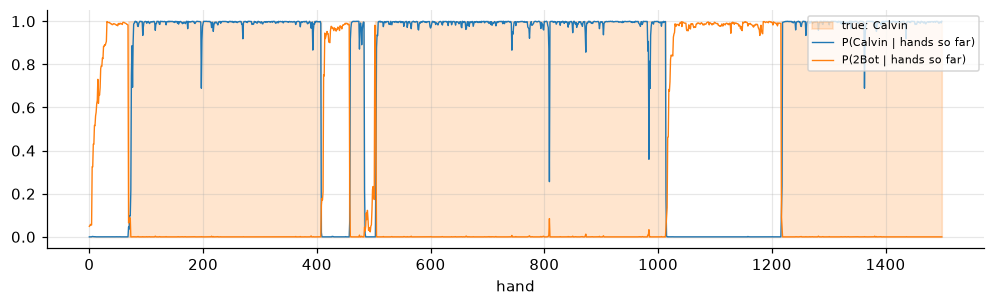
\includegraphics[width=0.85\textwidth]{figures/switch_detection.png}
\caption{Two programs glued into one sequence. Shaded: the second program is
playing. Lines: the network's probability for each program.}
\label{fig:switch}
\end{figure}

\paragraph{Playing whole hands.} We also let the model play complete hands
with a simple rule (fold below the pot odds, bet or raise when $q$ is high),
against copies of two ACPC programs: an aggressive one that bets or raises
61\% of the time, and a passive one that only checks and calls. Here the
results are not in the model's favour. Against the passive copy all agents tie.
Against the aggressive one, an agent that ignores the opponent's actions wins
22.7 chips per hand, and nothing beats it: the model of all opponents loses
$11.8\pm2.9$ chips per hand relative to it, because it reads the frequent bets
as strength and folds too often; learning online during the match recovers most
of this (only $1.9\pm1.6$ lower); the opponent's own model ties ($0.3\pm1.0$ lower). The same
pattern appears in the PettingZoo environment~\cite{terry2021}. The lesson is
that a model of the wrong opponent is expensive, and that learning on the fly
limits the damage. These tests are small and the betting rule is crude.

\paragraph{Humans change style.} On the IRC hands, models with two or three
styles predict test hands better than one style. The learned switch chance is
about $0.02$ per hand, a change every 50 to 65 hands, against one every 700
hands for the programs. The styles differ mostly in aggression (23\%, 31\% and
64\% bets and raises). A big loss raises the switch chance by only
$0.005\pm0.005$, so we cannot say that losing makes people change style.

\section{Conclusion}

Modelling an opponent as a Bayesian network over cards, strength, actions and
style lets every hand count, including the many where the cards stay hidden.
Ignoring those hands is a real mistake: the learned behaviour ends up about 80
times further from the truth. With folded hands included, the network reads
cards better, makes better river decisions when it is fitted to one opponent,
explains its advice, spots a new opponent within about ten hands, and finds
that humans change style often.

It does not yet win more over whole hands, and a model of the wrong opponent
can lose heavily. The strength groups are coarse, and the decision gain is far
from what perfect information would give. All checks need logged cards; in
human play a loser may hide their cards, which breaks
Proposition~\ref{prop:ignore} unless showing is modelled too. Next steps are a
smarter betting rule, finer strength features, and human data with full card
logs.

\bibliographystyle{plainnat}
\bibliography{refs}

\end{document}
